\chapter{Background}
\label{background}

In this section we first present an overview of the theoretical items necessary to our task of generating natural language from code features.
% In particular we cast our sequence generation problem in the commonly used framework of machine translation, exploring language models, translation techniques, and neural approaches to them. 
In particular we explore the commonly used framework of machine translation, covering language models, translation techniques, and neural approaches to them. 
We finally present an overview of the features of code that differentiate it from natural language, and conclude with a review of relevant work in the field.

\section{Introduction to Language Generation} % (fold)
\label{sec:lstm}

\subsection{Language Modelling} % (fold)
\label{sub:recurrent_neural_networks}

% In order to accurately model sequences of words, we often require an  require an evaluation of the true probability of distribution sequence of words.
Although natural language has the potential to be rich and complex, more often than not it is mundane and repetetive \cite{hindle_naturalness_nodate}. 
It is such repetitiveness that makes it possible to predict in many instances. For instance, in natural English the phrase ``\textit{The music is loud, turn it ...}", is much more likely to be followed by `\textit{off}', or `\textit{down}', than the word `\textit{around}'.
This is because the actual distribution of utterances is very sparse in  the vast space of possible utterances for a natural language.

In our task, we seek to generate sequences of natural language, $\{y_1, y_2,..., y_n\}$ from a set of features of code, $\mathcal{C}$.
Ideally we seek to do this through maximising a probability:

$$p(y_1, y_2,...,y_n | \mathcal{C}) = p(\{y_i\}| \mathcal{C}) \propto p(\mathcal{C} | \{y_i\})  p(\{y_i\})$$

where the last proportionality follows from Bayes' rule.
This $p(\{y_i\})$ term in this equation represents the probability of the sequence occuring naturally in the language. This term is what typical language models aim to represent.

Language models are an unsupervised means of determining the natural distribution of utterences in a language (or corpus). 
Often these utterences are broken down into single token sequences, and the probabilities are formed as a product of conditional probabilities.

$$p(y_1, y_2,...,y_n ) = p(y_n | y_1, y_2,...y_{n-1} )  p(y_1, y_2,...y_{n-1} )$$
$$= p(y_n | y_1, y_2,...y_{n-1} ) p(y_{n-1} | y_1, y_2,...y_{n-2} )...p(y_1)$$
$$ = \prod_{i=1}^{n} p(y_i | y_1^{i-1} ) $$ where $y_1^{i-1} =  \{y_1, y_2,...y_{i-1}\}$, the sequence of tokens from $1$ to $i-1$

These probabilities can be calculated in different ways, or under different assumptions. An n-gram model assumes a Markovian conditional independence structure, where the next token is conditionally independent of all others, given the previous $n$: 

$$ y_t \CI y_1^{t-n} \mid y^{t-1}_{t-n+1} $$
$$\therefore p(y_t | y_1, y_2,..., y_{t-1} )  = p(y_t | y_{t-n}, y_{t-n+1},..., y_{t-1}  ) $$

These then models estimate maximum likelihood probabilities from counts of occurences in models, and sometimes `smooth' these probabilities to overcome the sparsity of their training data.

Other models, such as neural language models, do not make such conditional indepence assumptions and use a neural network as a function approximator, instead of taking counts.
In our work, we effectively seek a conditional language model, which we can sample given our conditioning code features $\mathcal{C}$. As such, we draw inspiration from them for the architectures of our models.

\subsection{Conditional Generation of Language}

Many tasks in natural language processing require the generation of natural language conditioned on observations.
We draw on the work of many of these task, in our approach to our specific problem.
In this section we briefly overview three main conditional sequence generation tasks, comparing similarities with ours.

Firstly we consider machine translation. In this field, the objective is to generate the most likely sequence of a target language, $\{y_1, y_2,..., y_m\}$, given a sequence in an origin language  $\{x_1, x_2,..., x_n\}$. 
The translation seeks to maximise the probability:

$$ p(y_1, y_2,..., y_m| x_1, x_2,...,x_n )$$
The history and context of machine translation traditionally revolves around $\{y\}$ and $\{x\}$ being languages with the same semantic meaning. 
In this respect our task is not a typical translation task.
However, many models pioneered in this field are highly transferrable to any task aiming to condition one sequence upon another.

Secondly, the task of summarization aims to extract summaries or descriptions from a document.
Typically this involves extraction and/or abstraction of a document in the same modality or language.
Our task, extracting summaries about an element of a code document, naturally involves two distinct modalities - code as input, and english as output.
However, we desire our descriptions to somehow reflect a true and relevant summary of the argument, in the best case.
Therefore, although ours is not a typical summarization task, there are similarities that can highlight helpful potential approaches.

A final task with a parallel to ours is that of captioning. 
The distinction from summarization in this case is that captioning involves generating text from differnet modalities - such as captioning a picture, or video clip.
There parallels are here with both summarization, and our task, though it is perhaps unfair to describe documentation of code as `caption' when it aims to be a succinct description of only the most important parts of the code.

In summary our task falls in between a number of traditional NLP tasks and consequently related tasks blur the boundaries of translation, summarization and captioning. In the next section we present an overview of the relevant theoretical components for our model, indicating their provenance from their respective fields.

\section{Neural Approaches}

Given the maturity and prominence of the topic \footnote{Quote someone}, we assume a basic familiarity with neural networks, including linear and sigmoidal layers, multilayer perceptrons, and the backpropagation algorithm. For those seeking a further background on this topic, we recommend a number of books \cite{nielsenneural} \cite{Goodfellow:2016:DL:3086952} 


\subsection{Recurrent Neural Networks} % (fold)
\label{sub:recurrent_neural_networks}

Much of the semantic meaning of language is captured in the order of words. 
% It is not only the lexical tokens, but the sequence of them, that carries the information of a sentence.
This order can stretch beyond sentences, as context too can change the meaning of a sentence or phrase.
Vanilla neural networks such as multilayer perceptrons are poorly suited to capturing such long range information, as they are unable to remember preceding tokens in a sequence. 
Furthermore, they struggle from problems of vanishing and exploding gradient when processing long sequences \cite{bengio_learning_1994}.

A recurrent neural network (RNN) is one in which a hidden state is maintained by the network, while processing a sequence.
This hidden state allows information from previous tokens to propagate inside the network and contextualise the processing of future tokens.
Such networks have proved highly adaptable to language tasks, and enjoy widespread use within many sequence learning settings\cite{lipton_critical_2015}.

An example of an RNN used in our research is that of the Long Short Term Memory Unit (LSTM)\cite{hochreiter_long_1997}. These comprise of three gating mechanisms, ($f_t, i_t, o_t$), operating on the input $\mathbf{x_t}$ and state vectors $\mathbf{c_t}$ and $\mathbf{h_t}$
\cite{noauthor_understanding_nodate}. Each gating mechanism has a corresponding weight matrix, $W$, and bias vector $\mathbf{b}$, and operate according to the following equations:

\begin{equation}
    \mathbf{f_t} = \sigma(W_f [\mathbf{h_{t-1}}, \mathbf{x_t}] + \mathbf{b_f})
    \label{eq:lstm1}
\end{equation}
\begin{equation}
    \mathbf{i_t} = \sigma(W_i [\mathbf{h_{t-1}}, \mathbf{x_t}] + \mathbf{b_i})
    \label{eq:lstm2}
\end{equation}
\begin{equation}
    \mathbf{o_t} = \sigma(W_o [\mathbf{h_{t-1}}, \mathbf{x_t}] + \mathbf{b_o})
    \label{eq:lstm3}
\end{equation}
\begin{equation}
    \mathbf{\tilde{c_t}} = \text{tanh}(W_c [\mathbf{h_{t-1}}, \mathbf{x_t}] + \mathbf{b_c})
    \label{eq:lstm4}
\end{equation}
where [,] operator indicates concatenation and $\sigma$ indicates point-wise sigmoidal function.

These gating equations then combine to update the cell state $\mathbf{c_{t-1}}$ and the hidden state $\mathbf{h_{t-1}}$ as follows: 
\begin{equation}
    \mathbf{c_t} = \mathbf{f_t} * \mathbf{c_{t-1}} + \mathbf{i_t} * \mathbf{\tilde{c_t}}
    \label{eq:lstm5}
\end{equation}
\begin{equation}
    \mathbf{h_t} = \mathbf{o_t} * \text{tanh}(\mathbf{c_t})
    \label{eq:lstm6}
\end{equation}

where  $*$ indicates point-wise multiplication, and tanh indicates point-wise hyperbolic tan.

Interpretting these operations gives a good insight into the success of the LSTM.  
Equation \ref{eq:lstm1} represents the creation of a `forget' gate, where vector $\mathbf{f_t}$ represents what fraction of each dimension of $\mathbf{c_{t-1}}$ to retain. 
Equation \ref{eq:lstm2}  creates an `input' gate, where vector $\mathbf{i_t}$ represents what fraction of each dimension of our transformed input $\mathbf{\tilde{c_{t}}}$ we want to retain.  
$\mathbf{\tilde{c_{t}}}$ itself is created in equation \ref{eq:lstm4}. With both the `input' and `forget' gate, the  the cell state is updated in \ref{eq:lstm5}. 
The new hidden state $\mathbf{h_{t}}$ then derives from this cell state, which is modified by the output gate $\mathbf{o_t}$. 
Both $\mathbf{c_{t}}$ and $\mathbf{h_{t}}$ pass forward to the next time step, while $\mathbf{h_{t}}$ is also out put by the cell. 
A diagram is presented in Figure \ref{fig:lstm_colah}

\begin{figure}[tb]
    \centering
    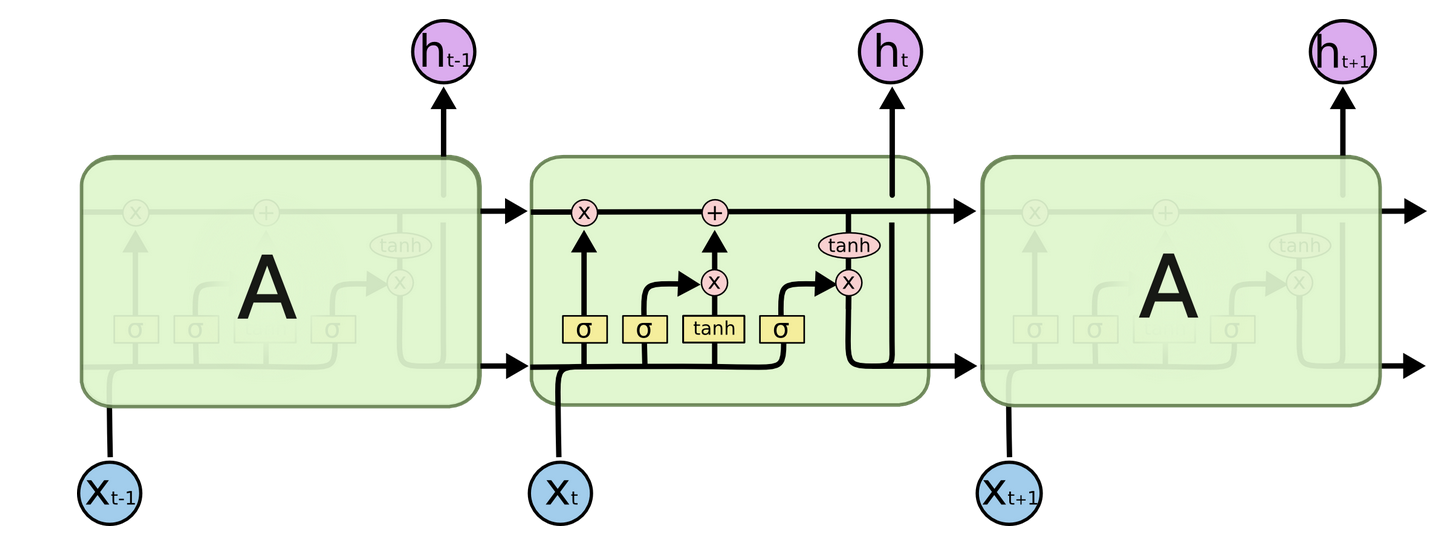
\includegraphics[width=\linewidth]{ModelPics/LSTMcolah.png}
    \caption{A diagram of an LSTM, sourced from \cite{noauthor_understanding_nodate}}
    \label{fig:lstm_colah}{}
\end{figure}

LSTM's have shown a remarkable versatility and strength in NLP tasks, not least in language modelling. A remarkable study of language modelling in 2017 showed that well-tuned LSTM architectures still surpass more recent and complex architecture, and can achieve state of the art results, despite their simplicity\cite{melis_state_2017}.

There also exist other forms of RNN units. The Gated Recurrent unit \cite{cho_properties_2014}, is another recurrent network unit that aims to simplify the LSTM, and has shown comparable performance to the LSTM in tasks such as speech signal modelling and music modelling \cite{chung_empirical_2014}.
However, for the purposes of our investigation, we use the LSTM for all recurrent units.

%BIDIRECTIONAL LSTMS??

\subsection{Sequence to Sequence Architectures} % (fold)
\label{sub:sequence_to_sequence_architectures}

At each time step, an RNN unit accepts an input $\mathbf{x_t}$ and emits an output $\mathbf{h_t}$. In the translation context, this 1-to-1 mapping of input to output is the equivalent of translating a sentence before you hear the end of it. For languages such as German, where the verb comes at the end of the sentence, this is almost impossible.

The sequence-to-sequence architecture, originally proposed by Sutskever et al \cite{sutskever_sequence_2014}, overcomes this limitation by processing the whole input sequence before translation even begins. 
In this framework, presented in figure \ref{fig:seqtoseq}, an rnn unit such as an LSTM acts as encoder, through which all word tokens are passed. Then the final hidden states of the encoder cell are used as the initial states of a decoder rnn cell.

This decoder is then used to sequentially generate a series of tokens, by conditionally choosing the word after its input. First a "start-of-sentence" token is fed in, generating a distribution over the vocabulary in the target language. The most likely word is the chosen, and fed back in to the  decoder, to generate a distribution of the next word. This method repeats until the sequence terminates, perhaps with a termination token).

In effect this results in a greedy form of decoding, where the most likely next word is continually selected from the decoder.  Other methods seek to explore the broader space of translations, by feeding in multiple tokens and retaining only the most likely sequences. This is known as beam search.

This architecture has found great use in machine translation, though it has some drawbacks. It has been shown that as the source sequence gets longer, the performance of the model worsens significantly \cite{cho_properties_2014}. This is partly due to the fact that model must now compress more information into the intermediate vector passed between encoder and decoder. A common way of dealing with such an issue is to use attention, as described in the next section. 

% What are the problems: long sequences
% Forgetful of what happens at the beginning - bi rnns
% Application to machine translation. 
% Raw code tokens to language - limited success

\begin{figure}[tb]
    \centering
    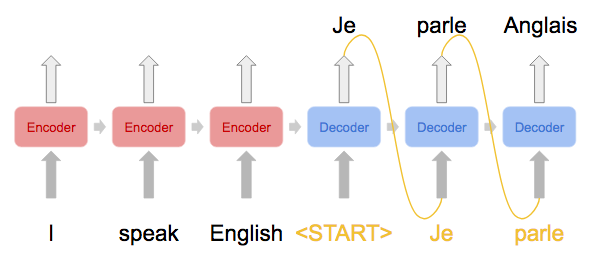
\includegraphics[width=\linewidth]{ModelPics/seq2seq.png}
    \caption{An example of sequence to sequence architecture}
    \label{fig:seqtoseq}
\end{figure}

\subsection{Attention} % (fold)

As the sequences get longer, encoder-decoder architectures struggle to pass the full information required from the encoder to the decoder. 
One way of improving this is to augment the decoder with a contextual vector at each step (see figure \ref{fig:attention})
As before, the decoder estimates the conditional probability for the next word $y_t$, given the input sentence $\mathbf{x}$, and previous output tokens ${y_1, ..., y_{t-1}}$.
 However, this changes from being a function of simply the input token, $y_{t-1}$, and hidden state, $s_{t}$ at step $t$:
\begin{equation}
p(y_t| y_1, ..., y_{t-1}, \mathbf{x} ) = g(y_{t-1}, s_t)
\end{equation}

to now being a function of the context vector at that point $c_t$ aswell:
\begin{equation}
p(y_t| y_1, ..., y_{t-1}, \mathbf{x} ) = g(y_{t-1}, s_t, c_t)
\end{equation}

The context vector at each step is itself calculated using a weighted sum of the rnn outputs $\{h_1,... h_{t_1}\}$:

\begin{equation}
c_t = \sum_{j=1}^{T_x}\alpha_{tj}h_j
\end{equation}
where
\begin{equation}
\alpha_{tj} = \dfrac{\text{exp}(a(s_{t-1}, h_j))}{\sum_k^{T_x}\text{exp}(a(s_{t-1}, h_k))}
\end{equation}
and $a$ is a function that maps to the reals - often a multilayer perceptron that is trained simultaneous to main training. 

This method was introduced by Bahdenau et al \cite{bahdanau_neural_2014} who demonstrated that the networks could use the attention to align words during translation.
In this case the $\alpha$ parameter acts like a weighting indicating the most important word used in each token generation - which word the decoder should pay attention to.

Variations on attention have found great use in the field of machine translation  \cite{luong_effective_2015}, and have even demononstrated their use independently of RNNs\cite{}. However they also have demonstrated their effectiveness in fields such as captioning, where they prove an effectve way of working with different modalities.

% [Xu et al.2015] Kelvin Xu, Jimmy Ba, Ryan Kiros, Kyunghyun Cho, Aaron C. Courville, Ruslan Salakhutdinov, Richard S. Zemel, and Yoshua Ben- gio. 2015. Show, attend and tell: Neural image cap- tion generation with visual attention. In ICML

In our models we use attention mechanisms extensively, both as a means of dealing with particularly long sequences (in our case of characters), and also as a means of dealing with the difficult modality of code.


\subsection{Distributed Representations} % (fold)
\label{sub:embeddings}

The vocabulary of natural language is vast and nuanced. 
Some words may appear very different lexically yet have similar semantic meaning - for instance `big' and `large'.
Others may appear lexically similar, but have different meanings - `large' and `largesse'. 
In our language generation tasks we wish to generate words that have the correct semantics.
As such it would be helpful to find numerical representations of words that reflect their semantic meaning.

One way of doing this is to distribute the semantic meaning over various components of a vector in a high dimensional space. Although such an idea is old 
%\cite HINTON 1984


% WHERE DO I CITE LUONG

\begin{figure}[tb]{}
    \centering
    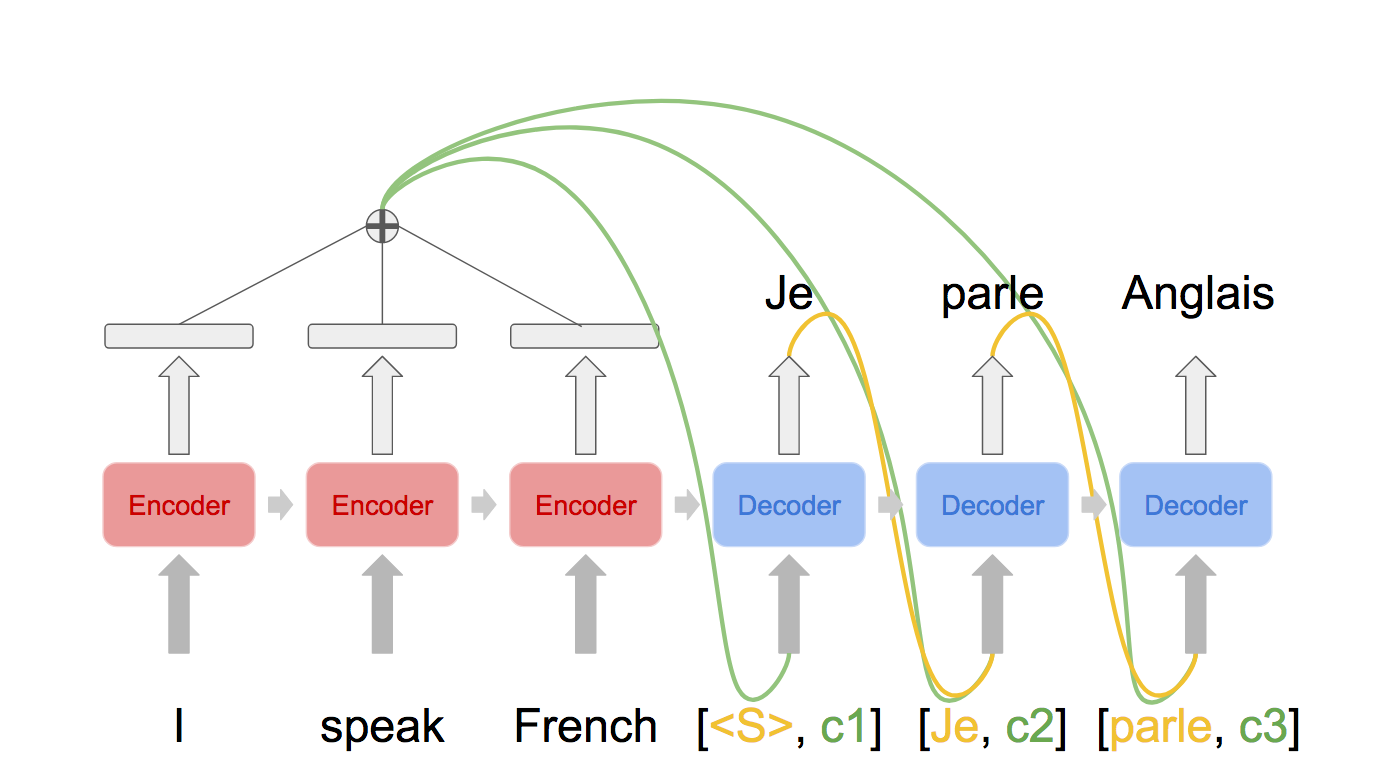
\includegraphics[width=\linewidth]{ModelPics/attention3.png}
    \caption{An example of sequence to sequence architecture with attention}
    \label{fig:attention}
\end{figure}




\section{Introduction to Source Code Structure} % (fold)
\label{sec:translating_code}

\subsection{Function Declarations} % (fold)
\label{sub:function_declarations}

\subsection{Abstract Syntax Trees} % (fold)
\label{sub:abstract_syntax_trees}

\subsection{Representations of Trees}

\blindtext

\section{Related Work in Source Code Modelling}

As mentioned in the Introduction, it is only through the recent development of large open source datasets that statistical approaches to code related tasks have been available to machine learning researchers. 
As would be expected of any new and growing field, the range of attempted tasks is still expanding. 
Although as of writing no formal attempt has been made to translate fine grained elements of source code into their natural language descriptions, a great deal of relevant insight has been made in the related fields of source code summarization, variable naming, documentation generation, and code language modelling. Many of these problems highlight possible approaches to modelling the patterns and structure of code as language, and can even be cast into a machine translation framework.  

In this review we summarise the current advances of these methods and how they relate to the task at hand.  We start by examining with the general progress in the language modelling of code, before moving on to specific tasks that can be posed as sequence generation tasks, such code comment prediction, code summarization or function naming. We subsequently examine advance in the related fields of representation of programs, before we finally examine the existing datasets, and the scope of the problems they are suitable to address. 

\subsection{Language Models of Source Code}

The earliest work modelling source code with natural language techniques comes from Hindle at al \cite{hindle_naturalness_nodate}, who used simple Kneser-Ney smoothed n-gram models of code tokens, to create language models for large-scale Java and C projects.
With these models, Hindle was able to demonstrate that the cross-entropy of source code within projects was lower than that of large English corpora - indicating the presence of repetetive common patterns that could be leveraged for code completion, naming and summarization.
This was consistent with findings by Gabel and Su \cite{gabel_study_2010} who examined the lines of approximately 6000 projects of code and found widespread repetition of sections of up to several lines, both within and across projects.
Despite the simplistic Markov chain assumption implicit in the ngram model, the effectiveness of this modelling techniques, especially within projects, opened up the field of code analysis to the wider natural language processing community.

This model, which only took into the lexical structure of code, was subsequently improved by Nguyen et al\cite{nguyen_statistical_2013}, who integrated semantic information into the n-gram model.
Instead of training on the raw string of the token, the \textit{lexeme}, this model condensed information such as data type, scope, role (such as literal, variable, function call) into a \textit{sememe}, and trained an n-gram topic model, modelling both local context \textit{sememes} ngrams, and global trends in the code.
This highlighted the value of taking into account the semantic information in code, as well as the lexical, in future prediction tasks.

Since then a number of different language models of code have formed, largely finding their use in code completion tasks. These are often most successful if they can take into account the long range dependencies of code, or elements of the code beyond simple lexical structure. For instance Tu et al added a cache mechanism to improve Hindle's ngram model in capturing long range dependencies  \cite{tu_localness_nodate}, while this itself was surpassed (up to 9 grams) with a basic recurrent neural language model by White et al\cite{white_toward_2015}.
Most recently, Bhoopchand et al used a sparse pointer network to create a language model that significantly outperformed a LSTM baseline on code completion tasks, that was able to refer to objects in code over 60 tokens previous\cite{bhoopchand_learning_2016}.

This work in language modelling has direct applicability to our task at hand, as it points out relevant strategies in picking out the statistically important features of `natural' code. In particular we note the importance of capturing long range dependencies (as seen in neural models), with the performance benefit that can be brought by taking into account semantic information (from the instructions given to the computer).

\subsection{Sequence Generation from Code}

Given the industrial importance of software engineers understanding sections of code, a long running task is that of code summarization. 
This task involves taking large sections of code blocks, and summarising its meaning in natural language. It has historically had parallels with the long running (inverse) problem of semantic parsing. CITE
As such, early approaches to this problem completely ignored the `naturalness' properties of code and its comments, and instead, automatic summarization of source code was tackled with rule-based methods. 

Work by Sridhara et al \cite{sridhara_[not_2010}  used static analysis to find important semantic subunits of code in Java projects, and used sets of sentence templates to produce English from these subunits.
% This model revolved around automatic rule-based summarization of the source code in the source code in consideration.
This work produced text that describe the functions in question to a high degree of accuracy, but Sridhara noted the potential lack of transferrability to other settings, and lack of examples with which to compare their summaries.  
This procedure was also inherently inflexible, relying on human crafted templates, and specified rules. Furthermore the size of the dataset, four projects in total, indicated a potential problem in the generalisability of the work to other domains, projects or even languages.

However, the advent of the statistical approaches to code language modelling led by Hindle et al \cite{hindle_naturalness_nodate} signalled the start of similar approaches to sequence generation. The earliest is Movshovitz-Attias et al \cite{movshovitz-attias_natural_nodate}, who used both ngrams and topic models such as LDA to predict comments from JAVA source code. In this they found that modelling the lexical components of source code as coming from a mixture of topics - "code" and "text" - outperformed models that ignored this distinction.  This pointed to the strength of taking into account features of code (such as distinguishing comments from commands), even if such destinction were still purely on the lexical level.

% Since then, statistical approaches have become more popular in attacking the problem, often involving much larger corpora of training data.
% Iyer et al \cite{iyer_summarizing_2016} sourced a large dataset of code snippets and questions from Stack Overflow, a popular programming website, to attempt this problem statistically.
Since then neural models have become popular methods of attacking sequence generation, as they capture long range dependencies in sequences, and have shown great promise in other neural translation tasks.

A particularly successful example is that of Iyer et al \cite{iyer_summarizing_2016}, who applied a neural attentional model to the problem of generate code summaries, training on a large collection of snippets and questions from the Stack Overflow.   Their model combined two features: a distributed representation of the code, generated by an attentional mechanism \cite{luong_effective_2015} over code token embeddings; and a Long Short Term Memory unit \cite{hochreiter_long_1997} to encode natural language tokens. Together these generated descriptions as a sequence of conditional distributions, in an encoder-decoder model. 

Specifically this model calculated the probability of generating a length $l$
descriptive sequence through a product of conditional probabilities the previous $l-1$ tokens

$$P(\{n\}_1^l) = \prod_{i=1}^lp(n_i | n_1, ..., n_{i-1} ) $$

where each conditional probability was the proportional to a non-linear transformation of the combination of hidden state of the LSTM $\mathbf{h_i}$ and the attentional vector  $\mathbf{t_i}$ at that point in the sequence: 

$$\text p(n_i | n_1, ..., n_{i-1} ) \propto \mathbf{W}\text{tanh}(\mathbf{W_1h_i} + \mathbf{W_2t_i})$$

where $\mathbf{W} \in \mathbb{R}^{|N|\text{x} H}, \mathbf{W_1}$ and $\mathbf{W_2} \in \mathbb{R}^{H \text{x} H}$  and $ H$ is embedding dimensionality of words, $ N $ the vocabulary.\cite{iyer_summarizing_2016}
A visual schematic of the model is preseted in Figure \ref{fig:Iyer}.
Iyer et al then ran a beam search over the decoder to explore the space of likely sequences, and evaluated their generations using the BLEU-4 and METEOR metrics.

This model achieved a new record in the performance of the code summarization task, and outperformed rival NLP models such as MOSES, a traditional phrase-based machine translation model \textbf{CITE \& paraphrase}, and SUM-NN, another attention based summarization model using dense layers instead of LSTMs.CITE. It also achieved a first in learning to generate original sentences from arbitrary code sections, and has proved successful in other domains.  

Loyola et al \cite{loyola_neural_2017}, for instance, adapted a similar attention model to Iyers to generate short descriptions of differnces in code.
This time intead of training on a single piece of source code and questions, data was sourced to present pairs of code changes, `diffs', with comments describing the change, `commit messages'. 
In this setting, the attentional model was able to generate faesible messages, both within projects and between projects.

Both these attention models showed the effectiveness of being able to pickout relevant portions of code at different points in sequence generation, but failed to take into account the longer term correlations of the tokens in source code. In fact by only using this kind of attentional model to process source code, both models treat the source code as little more than bag of token embeddings.

In this regard, an improvement on these attentional models is that Alamanis et al \cite{allamanis_convolutional_2016}, which uses a convolutional attention network over tokens, for the task of predicting the names of functions given their body. 
%aiming to capture long range correlations in code through spatial convolutions instead of temporal hidden state.

In this model source code is split lexically in to a padded sequence of embedded tokens, over which a one dimensional convolution of fixed width is run, to create a number of attentional feature vectors $\mathbf{\{v_k\}}$.
These feature vectors are then point-wise multiplicatied with the hidden state of an rnn, $\mathbf{h_{t-1}}$, to be effectively `selected' for their relevance to next generated token, before being normalised.

This set of feature vectors is then convolved with an attention kernel, to give a set of attention weights, each corresponding to a token embedding. 
A final attention vector $\mathbf{\alpha}$ is constructed from the convex combination of the token embeddings under the attention weights, and this vector is used to generate a distribution over the next function subtoken.
An illustration of the algorithm with pseudo code is presented in Figure X.

The authors of this model apply it to both the narrow task of generatign function names, and that of code retrieval. In it they find that taking into account the long range features of the code in the convolutional model surpasses a baseline attentional model of the machine translation model originated by Bahdenau \cite{bahdanau_neural_2014}, and found that this performance was further improved by adding a cacheing mechanism to the model.

Both these attention models show the strengths that attention can provide in combining the modalities of text and code. However, a key failing of both models remains their lack of appreciation for the syntax and semantic of the underlying code.
Although Allamanis et al's model is more aware of the structure of lexical code tokens than Iyer et als, both models continue to ignore a fundamental channel of information communication through code - that of communication from human to computer.

% Other forms of machine translation? 
% Phrase based translation, 
% neural mthods, 
% pseudo code

As of writing no published work has been applied to generating documentation of source code using the syntactical structure of source code.  However, a number of pieces of work have recently started to examine such structure in other tasks. These are the topics of the next section of review.

\subsection{Representations of Code}

As mentioned previously, most work in the field of statistical analysis of code has focused on the lexical tokens of code. 
* These can be different, same meanining, miss the underlying AST
* Recently a number of of tasks have aimed to make use of different aspects of code flow:
* Program embeddings 1, 2, 
* Graphs
* Code2Vec

\section{Existing Datasets}

The scope of the tasks available to challenge researchers is naturally limited by the set of available datasets.
In a field as young as that of sequence generation from source code, there is still a limitation in the number of datasets that have been collected, cleaned and are suitable for certain tasks.
In this section we outline the current state of the available datasets, indicating why none so far is suitable the task of translation of fine grained elements of source code.

\subsection{Language Modelling Corpora}
An early, prominent corpus of data is the GitHub Java Corpus, by Allamanis and Sutton\cite{allamanis_mining_2013}. This corpus is composed of 14,800 open source Java projects, with over 350 million lines of code (LOC), and is approximately two orders of magnitude larger than the original dataset of Hindle et al. This dataset is rich and a good example of a dataset highly suited to language modelling, but is of little use for natural language problems, given how poorly documented much open source code is.
Similar language modelling corpora exist in other languages, and run in to the same problem. Bhoopchand et al \cite{bhoopchand_learning_2016} focus on high quality code, by pulling large sections of Python code from projects with more than 100 stars from GitHub, finally collecting 40 million LOC. 
Despite the quality and scale of this corpus, the lack of structured language surrounding the code makes it unsuitable to our translation tasks, let alone anything as fine grained as we would wish.

\subsection{Django Dataset}



\subsection{Stack Overflow Dataset}

A commonly used dataset for code captioning and summarization tasks is sourced from a large corpus of questions and code snippets from the programming help website Stack Overflow, as generated by Iyer et al\cite{iyer_summarizing_2016}. In it, questions such as ``how do I concatenate entire result sets in mysql? ' are paired with the snippets of C\# or SQL which are responses to the question, posted by other users online.
Although widely used, this dataset suffers from a number for undesirable features for our task. 

First of all the preparation of such a dataset demonstrates a lot of arbitrary cleaning.
Since many of the responses from the website are invalid or do not quote code, the snippets in question have been found by searching for html \mintinline[]{python}{<code>} tags in the upvoted answers. 
The authors note that these sections of code often bore no real relevance to the question at hand. Therefore the authors were forced to train a semi-supervised classifier to filter only relevant snippets to the question at hand.
This convoluted pipeline runs the risk of increasing the number anomalous datapoints in the dataset, whilst reducing almost a million (query,snippet) pairs from each language, down to 66,000 pairs  of C\# and 32,000 pairs of SQL.

Furthermore, the authors noted that often the informal code snippets often contained syntactic errors, with only 12\% of SQL snippets parsing without syntactic error. They progress with a best-effort parse, but this
 lack of code quality, naturally poses a problem for our fine grained analysis of code segments, or indeed any analysis using the syntactical properties of code.

Finally the dataset itself lacks a lot of the context and information needed for the granular analysis necessary for individual sections of code. Not only is the natural language not tailored to specific parts of the code, but the artificial snippets lack a lot of the context of real `natural' codebases. In fact, given the snippets' only relevant context is that of the question, the authors are forced to mask items like string literals and the like, to prevent the close context of the question and nothing else. This modification of the code is also undesirable.

Naturally in our search for an appropriate code base, we seek larger bigger elements of `real' (and fully parsing) code, with appropriate descriptions of elements, and a greater sense of `naturalness'.

\subsection{Edinburgh Corpus}

A recent corpus specifically tailored to code-to-text generation, is one of Python code as released by Barone and Senrich \cite{barone_parallel_2017}, which we refer to as the Edinburgh Corpus. 
This is a set of 109,000 triplets of function declarations, bodies, and documentation strings (docstrings), scraped from the most popular projects in GitHub, using the same methodology as Bhoopchand et al. 

In this dataset, the authors focus on finding real world code, and extracting the string, written by code authors, providing a description of each function.
Although these source code sections and natural language strings are more `natural', than their Stack Overflow counterparts, they still don't suit our needs, mainly in the form of the language they provide. 

Python's documentation strings are designed to be an explicit guide as to how to use the function. 
For any method in python, calling the built-in \mintinline[]{python}{help} function will display this string to the user, with the function declaration. 
Therefore this string often presents an overall view of the function, with very little reference to the inner workings of the code. 
This follows from abstraction principles of keeping library api's as a black box.
In fact from a code-readers perspective (instead of a code-users perspective), the most informative section of the docstring is where the arguments are described. 
Such a segment is not always present, but if so, would be perfect for our fine grained summarization task, as it links direct elements used in the code, to their natural-language descriptions. 

Only part of the Edinburgh corpus functions contain such such descriptions, and these are mixed in with the docstring as a whole, and therefore difficult to parse in whatever numbers they exist.
As such this makes the Edinburgh corpus limited to our needs.

% edinburgh
% django
% stack overflow


% These attentional style models have shown great success at combining the different modalities of text and code, and this particular model
\begin{figure}[tb]
    \centering
    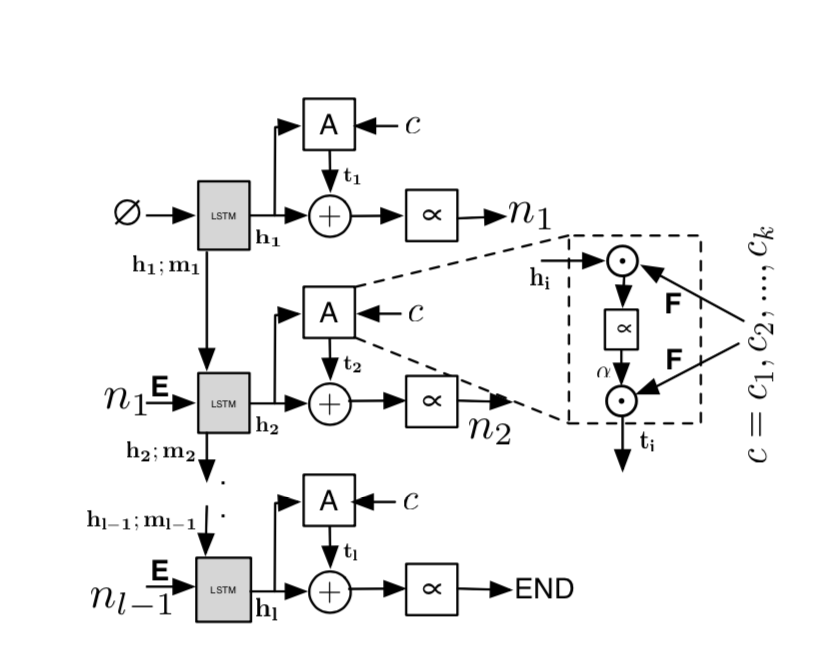
\includegraphics[width=0.5\linewidth]{ModelPics/Iyer_etal.png}
    \caption{Iyer et als Code NN, taken from \cite{iyer_summarizing_2016}}
    \label{fig:Iyer}
\end{figure}



